\chapter{Analyse af markbilleder} \label{sec:mark}
Denne sektion har til formål at klarlægge udfordringer ved korrespondanceanalysen af markbilleder. Udfordringerne opstilles på baggrund af en analyse af billederne og vil resultere i hypoteser om, hvilke korrespondanceanalytiske metoder, der bedst muliggør en korrekt korrespondanceanalyse.
\section{Flyverute}
<Dronens overflyvning foregår ved at dronen får fire punkter, der definere markens placering. Dronen starter derefter i et hjørne og flyver systematisk fra side til side for at overflyve hele marken. Dronen flyver med én orientering. Dronen starter med en højde på ca. 50 meter og taber derefter glidende højde til den er på ca. 6 meter.>
\section{Markbilleder}
Billederne består af tilfældige kornstrukturer med traktorspor indimellem. Som illustreret i figur <Indsæt billede der viser udsnit af korn>, er kornet af relativ identisk udseende, og det er derfor vanskeligt at differentiere imellem korn områder, da der ikke opstår definerbare mønstre. Ligheden imellem billederne kan derfor besværliggøre korrespondanceanalysen da det er svært at differentiere om to punkter korrespondere eller ej, hvilket gør det interessant at undersøge hvorvidt det er muligt at opnå korrespondancer.
 figur \ref{fig:korn}.
\begin{figure}[H]
    \centering
    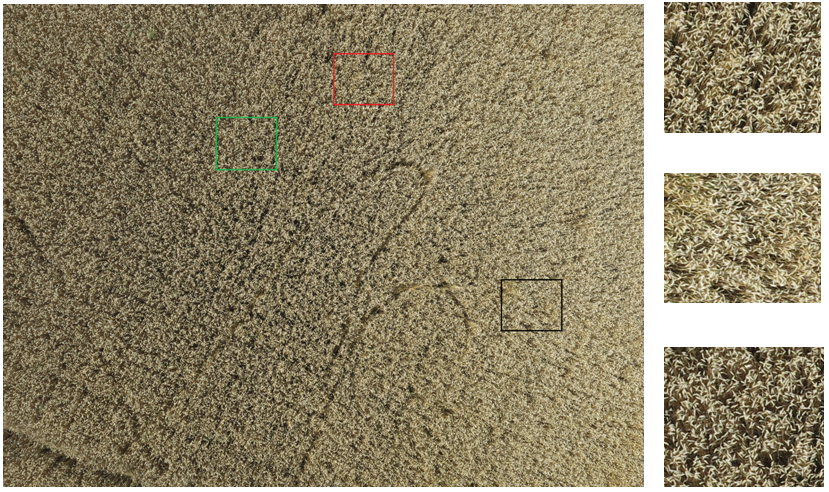
\includegraphics[width=0.65\textwidth]{fig/20.png}
     \vspace{-1em}
    \begin{center}    
       \caption{\textcolor{gray}{\footnotesize \textit{Markbillederne forstørret ind på enkelte korn.}}}
    \label{fig:korn}
     \end{center}
     \vspace{-2.5em}
  \end{figure} \noindent
Følgende observationer er gjort omkring markbillederne:
\begin{itemize}
\item{\textbf{Overlap:} Overlappet imellem billederne har en signifikant indflydelse på korrespondanceanalysen. Et stort overlap vil betyde at interessepunkter har større sandsynlighed for at indgå i begge billeder. Derfor, ved mindre overlap, skal der udvælges flere interessepunkter. Det er estimeret at billederne overlapper hinanden med ca. 70\%, der forekommer dog store udsving i overlappet, alt efter hvilken højde billederne er taget på. Figur \ref{fig:overlap} viser fire billeder, sat sammen parvist, der er taget ved to forskellige højder, hvor billedernes overlap er markeret med blåt. (a) er taget når dronen er på største højde, billederne er estimeret til at overlappe hinanden med ca. 80 $\%$. (b) er taget ved en lavere højde, billederne overlapper hinanden med ca. 35 $\%$.
\begin{figure}[H]
    \centering
    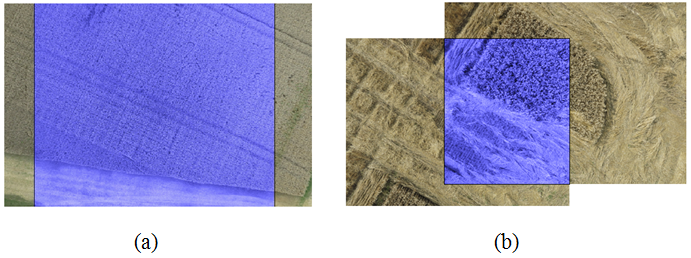
\includegraphics[width=0.65\textwidth]{fig/17.png}
     \vspace{-1em}
    \begin{center}    
       \caption{\textcolor{gray}{\footnotesize \textit{Markbilleder taget fra forskellige højde, det blå område indikere overlap.}}}
    \label{fig:overlap}
     \end{center}
     \vspace{-2.5em}
  \end{figure} \noindent }
\item{\textbf{Rotation:} Dronen rotere når den er nået kanten af marken og skal dreje, hvilket er illustreret i figur \ref{fig:rotation}. Denne rotation er ca. 10-15$^{\circ}$. Der forekommer også mindre uregelmæssige rotationer på 5$^{\circ}$.
\begin{figure}[H]
    \centering
    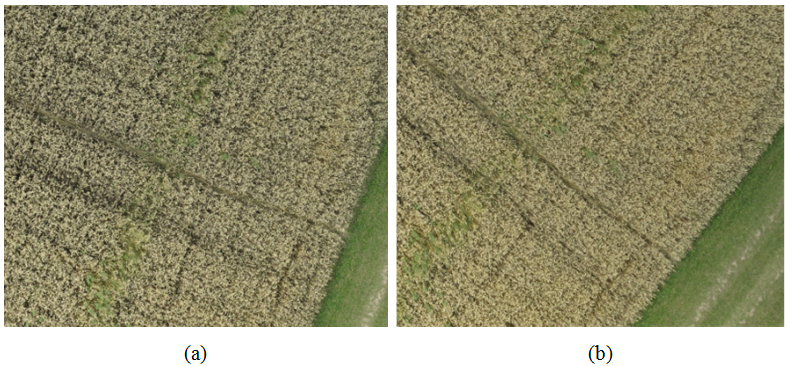
\includegraphics[width=0.65\textwidth]{fig/19.png}
     \vspace{-1em}
    \begin{center}    
       \caption{\textcolor{gray}{\footnotesize \textit{Dronen skal til at ændre retning, hvilket giver rotation i billederne.}}}
    \label{fig:rotation}
     \end{center}
     \vspace{-2.5em}
  \end{figure} \noindent}
\item{\textbf{Skala:} Kornet i markerne forekommer på samme skala ift. kameraet, da markerne er flade. Dronen ændrer dog højde under overflyvningen.}
\item{\textbf{Okklusion:}
Korn, der stikker direkte op imod kameraet, ses som mørke områder pga. den synlige jord, hvilket vil resultere i et mørkere område direkte under dronen. Forskydes kameraets position, vil det samme område nu ligne korn, da jorden ikke længere kan ses. sDette kan have en stor indflydelse på korrespondanceanalysen, da mørke områder kan opfattes som interesseområder, og medføre inkonsistente beskrivelser af interessepunkter.
\begin{figure}[H]
    \centering
    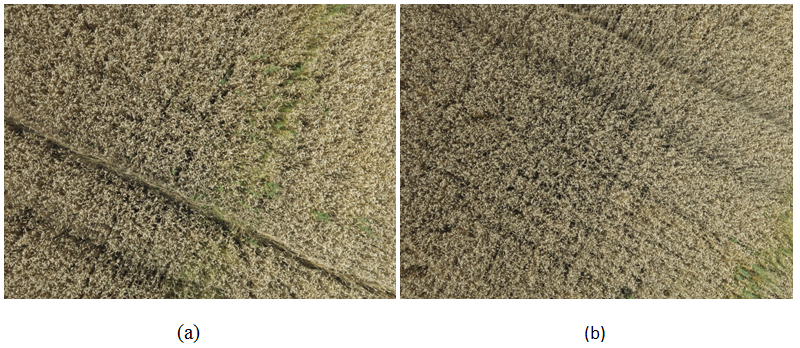
\includegraphics[width=0.65\textwidth]{fig/18.png}
     \vspace{-1em}
    \begin{center}    
       \caption{\textcolor{gray}{\footnotesize \textit{ To forkudte billeder, hvor traktorsporet er okkluderet. }}}
    \label{fig:okklusion}
     \end{center}
     \vspace{-2.5em}
  \end{figure} \noindent
Figur \ref{fig:okklusion} er et eksempel på okklusion af jord, hvor traktor spor optræder direkte under dronen og derefter forskudt. Traktorsporet, der optræder direkte under dronen, er tydelig og man se jorden. For det samme traktorspor, i det forskudte billede, er jorden ikke længere synlig. Det er også værd at bemærke at kornet, direkte under dronen, afgiver mørke områder. Denne okklusion forekommer umiddelbart kun når dronen er på lav højde.}
\end{itemize}
\section{Hypoteser}
Udefra ovenstående analyse er der opstillet følgende hypoteser om krav til de udvalgte metoder:
\begin{itemize}
\item{ <Det forventes, grundet strukturen af korn, at detektorer som leder efter veldefineret strukturer, som hjørner, ikke vil have en god effekt på korn, men at blobs vil give bedre resultater.> }
\item{ Det forventes ikke at metoderne behøver være rotationsinvariante, grundet den lille rotation der forekommer imellem billederne. }
\item{Det forventes at metoderne skal være skalainvariante, både pga. den skiftende fotograferingshøjde, men også for at tilpasse detektoren størrelsen som interesseområderne forekommer på.}
\item{Grundet det til tider lille overlap imellem billeder, forventes det at detektoren skal tilpasses til at finde mange punkter, for at sikre en repeterbar detektion.}
\end{itemize}